\chapter*{PRÉSENTATION DU PROJET AGRICULTURE CAMEROUN}
\addcontentsline{toc}{chapter}{PRÉSENTATION DU PROJET AGRICULTURE CAMEROUN}


\section{Description du Système}

\subsection{Contexte et problématique}

Le Cameroun, surnommé l'Afrique en miniature, présente une diversité agro-écologique remarquable avec ses dix régions aux caractéristiques climatiques et pédologiques distinctes. Cette richesse naturelle constitue à la fois un atout majeur et un défi complexe pour le développement agricole. L'agriculture camerounaise, qui emploie près de 70\% de la population active et contribue significativement au PIB national, fait face à des défis multidimensionnels qui freinent son potentiel de développement et limitent l'amélioration des conditions de vie des agriculteurs.

La \textbf{fragmentation de l'information agricole} représente l'un des obstacles majeurs. Les agriculteurs camerounais, particulièrement ceux des zones rurales, ont un accès limité aux informations essentielles pour optimiser leurs activités. Les données météorologiques précises et localisées restent largement inaccessibles, forçant les agriculteurs à se fier uniquement à leur expérience et aux signes traditionnels pour planifier leurs activités. Cette situation est exacerbée par l'absence de systèmes centralisés et accessibles pour diffuser les innovations agricoles, les bonnes pratiques et les alertes phytosanitaires.

Le \textbf{changement climatique} intensifie la vulnérabilité du secteur agricole camerounais. Les variations imprévisibles des précipitations, l'augmentation de la fréquence des événements climatiques extrêmes et les modifications des cycles saisonniers traditionnels perturbent profondément les calendriers agricoles établis. Les agriculteurs du Nord et de l'Extrême-Nord font face à des sécheresses plus fréquentes et sévères, tandis que ceux du Littoral et du Sud-Ouest subissent des inondations dévastatrices. Cette variabilité climatique croissante rend obsolètes de nombreuses pratiques traditionnelles et nécessite une adaptation rapide que la plupart des agriculteurs peinent à réaliser faute d'information et de moyens.

La \textbf{gestion inefficace des ressources} constitue un autre défi critique. L'utilisation non optimale de l'eau, des engrais et des pesticides entraîne non seulement des coûts de production élevés mais aussi une dégradation environnementale préoccupante. Les sols, surexploités et mal entretenus, perdent progressivement leur fertilité. L'absence de conseils personnalisés sur la gestion des intrants conduit à des pratiques inadaptées qui compromettent la durabilité des exploitations agricoles.

Les \textbf{pertes post-récolte et la volatilité des marchés} affectent gravement la rentabilité des exploitations. Sans accès aux informations sur les prix du marché, les tendances de la demande et les opportunités de commercialisation, les agriculteurs vendent souvent leurs produits à perte ou manquent des opportunités lucratives. L'absence de systèmes de prévision économique adaptés au contexte local empêche une planification stratégique des cultures en fonction de la demande du marché.

La \textbf{prévalence des maladies et ravageurs} représente une menace constante pour la productivité agricole. La pourriture brune du cacao dans les régions du Centre et du Sud, le flétrissement bactérien du bananier plantain dans le Littoral, ou encore les attaques de chenilles légionnaires sur le maïs dans l'Adamaoua causent des pertes considérables. Le diagnostic tardif ou erroné de ces problèmes phytosanitaires, combiné à l'utilisation inappropriée de traitements, aggrave les dégâts et augmente les coûts de production.

Face à ces défis interconnectés, il devient impératif de développer une solution technologique intégrée qui puisse fournir aux agriculteurs camerounais les outils et informations nécessaires pour transformer leurs pratiques agricoles, améliorer leur productivité et assurer la durabilité de leurs exploitations.

\subsection{Objectifs du système multi-agents}

Le système multi-agents Agriculture Cameroun a été conçu avec une vision ambitieuse : \textbf{démocratiser l'accès aux technologies agricoles modernes} pour tous les agriculteurs camerounais, des petits exploitants aux grandes coopératives, en créant un écosystème intelligent qui combine l'expertise locale avec la puissance de l'intelligence artificielle.

L'objectif principal du système est de créer un \textbf{assistant agricole intelligent et accessible} qui agit comme un conseiller personnel pour chaque agriculteur. Ce système vise à combler le fossé entre les connaissances agricoles de pointe et les pratiques sur le terrain, en fournissant des recommandations personnalisées, contextualisées et actionnables. L'approche multi-agents permet de décomposer la complexité du domaine agricole en expertises spécialisées tout en maintenant une cohérence globale dans les conseils fournis.

Le système poursuit plusieurs objectifs spécifiques interconnectés. Il vise d'abord à \emph{améliorer la prise de décision agricole} en fournissant aux agriculteurs des informations précises et opportunes sur tous les aspects de leur activité. Cela inclut des prévisions météorologiques localisées permettant une planification optimale des activités agricoles, des recommandations de cultures adaptées aux conditions spécifiques de chaque exploitation, et des conseils sur les meilleures pratiques culturales basées sur les dernières recherches agronomiques adaptées au contexte camerounais.

Un autre objectif crucial est la \emph{réduction des pertes agricoles} à travers un système de détection précoce et de diagnostic précis des problèmes. Le système permet l'identification rapide des maladies et ravageurs, propose des stratégies de traitement appropriées privilégiant les méthodes durables, et offre des conseils préventifs pour minimiser les risques futurs. Cette approche proactive contribue significativement à la sécurisation des récoltes et à l'amélioration des rendements.

L'\emph{optimisation économique} des exploitations constitue un pilier fondamental du système. En fournissant des analyses de marché en temps réel, des calculs de rentabilité précis et des stratégies de commercialisation adaptées, le système aide les agriculteurs à maximiser leurs revenus tout en minimisant leurs coûts de production. L'intégration d'informations économiques permet une planification stratégique des cultures en fonction des opportunités du marché.

Le système vise également à promouvoir une \emph{agriculture durable et respectueuse de l'environnement}. En optimisant l'utilisation des ressources naturelles, en recommandant des pratiques de conservation des sols et en favorisant l'adoption de techniques agroécologiques, le système contribue à la préservation de l'environnement pour les générations futures. Cette approche durable est essentielle face aux défis du changement climatique et de la dégradation environnementale.

L'accessibilité et l'inclusivité sont au cœur de la conception du système. En utilisant le langage naturel et en s'adaptant au niveau de connaissance de chaque utilisateur, le système s'assure que même les agriculteurs ayant une éducation formelle limitée peuvent bénéficier de conseils experts. La prise en compte des langues locales et des pratiques traditionnelles garantit une adoption large et efficace de la technologie.

\subsection{Bénéficiaires et impact attendu}

Le système Agriculture Cameroun a été conçu pour servir un large éventail de bénéficiaires dans l'écosystème agricole camerounais, avec des impacts spécifiques adaptés aux besoins de chaque groupe.

Les \textbf{petits exploitants agricoles} constituent le groupe de bénéficiaires prioritaire. Ces agriculteurs, qui cultivent généralement moins de 5 hectares et représentent la majorité des producteurs camerounais, bénéficieront d'un accès sans précédent à des conseils agricoles personnalisés. Pour eux, le système représente un changement paradigmatique, transformant des pratiques souvent basées uniquement sur la tradition en approches éclairées par des données scientifiques adaptées à leur contexte local. L'impact attendu inclut une augmentation significative des rendements grâce à l'optimisation des pratiques culturales, une réduction des pertes dues aux maladies et ravageurs grâce au diagnostic précoce, et une amélioration des revenus grâce à une meilleure compréhension des marchés et des opportunités de commercialisation.

Les \textbf{agriculteurs commerciaux et les coopératives} trouveront dans le système un outil puissant pour optimiser leurs opérations à grande échelle. Pour ces acteurs, l'impact se traduira par une planification plus précise des activités agricoles basée sur des prévisions météorologiques fiables, une gestion optimisée des ressources permettant des économies substantielles, et une capacité accrue à anticiper et répondre aux demandes du marché. Le système leur permettra également de standardiser les bonnes pratiques au sein de leurs organisations et d'améliorer la traçabilité de leurs productions.

Les \textbf{jeunes agriculteurs et entrepreneurs agricoles} représentent un groupe particulièrement important pour l'avenir de l'agriculture camerounaise. Pour cette génération technophile, le système offre une interface moderne et intuitive qui rend l'agriculture plus attractive et professionnelle. L'impact attendu comprend une augmentation de l'intérêt des jeunes pour les carrières agricoles, le développement de nouvelles entreprises agricoles innovantes, et l'émergence d'une nouvelle génération d'agriculteurs combinant savoir traditionnel et technologies modernes.

Les \textbf{agents de vulgarisation agricole et conseillers techniques} verront leur travail transformé et amplifié par le système. Au lieu de remplacer ces professionnels essentiels, le système agit comme un multiplicateur de force, leur permettant d'atteindre et d'assister un nombre beaucoup plus important d'agriculteurs. L'impact pour ce groupe inclut une amélioration de l'efficacité de leurs interventions, un accès à des informations actualisées pour enrichir leurs conseils, et la possibilité de se concentrer sur les cas complexes nécessitant une expertise humaine spécialisée.

Les \textbf{institutions gouvernementales et organisations de développement} bénéficieront d'un outil puissant pour la mise en œuvre et le suivi de leurs programmes agricoles. Le système peut collecter des données anonymisées sur les pratiques agricoles, les défis rencontrés et les tendances émergentes, fournissant ainsi des insights précieux pour l'élaboration de politiques agricoles basées sur des données réelles. L'impact attendu comprend une meilleure allocation des ressources publiques, une évaluation plus précise de l'impact des interventions, et une capacité accrue à répondre rapidement aux crises agricoles.

L'impact sociétal global du système s'étend bien au-delà des bénéficiaires directs. En améliorant la productivité agricole et les revenus des agriculteurs, le système contribue à la \emph{réduction de la pauvreté rurale} et à l'amélioration de la sécurité alimentaire nationale. La promotion de pratiques agricoles durables contribue à la \emph{préservation de l'environnement} et à l'adaptation au changement climatique. L'amélioration de l'attractivité du secteur agricole pour les jeunes contribue à \emph{réduire l'exode rural} et à dynamiser les économies locales. Enfin, en démocratisant l'accès à l'information agricole, le système contribue à \emph{réduire les inégalités} entre les différentes régions et catégories d'agriculteurs.

\section{Architecture du Système}

\subsection{Vue d'ensemble de l'architecture}

L'architecture du système Agriculture Cameroun repose sur une conception modulaire et distribuée qui maximise la flexibilité, la scalabilité et la maintenabilité. Cette architecture multi-agents orchestrée reflète la complexité du domaine agricole tout en offrant une interface unifiée et cohérente aux utilisateurs finaux.

Au cœur de l'architecture se trouve un \textbf{modèle d'orchestration hiérarchique hybride} qui combine les avantages d'une coordination centralisée avec l'autonomie des agents spécialisés. Cette approche permet une gestion efficace des requêtes complexes nécessitant l'expertise de plusieurs domaines tout en maintenant la réactivité nécessaire pour les requêtes simples. L'architecture est conçue pour être résiliente, avec des mécanismes de fallback et de récupération d'erreurs à chaque niveau.

La \textbf{couche d'interface utilisateur} constitue le point d'entrée unique du système. Elle accepte les requêtes en langage naturel, maintient le contexte conversationnel et présente les réponses de manière claire et actionnable. Cette couche utilise les capacités de traitement du langage naturel de Google ADK pour comprendre les nuances et les intentions des utilisateurs, qu'ils s'expriment en français, en anglais ou même en mélangeant les langues comme c'est souvent le cas au Cameroun.

L'\textbf{Agent Coordinateur Principal} agit comme le chef d'orchestre du système. Il analyse chaque requête utilisateur pour identifier les domaines d'expertise nécessaires, décompose les requêtes complexes en sous-tâches spécialisées, et coordonne les interactions entre les différents agents. Cet agent maintient une vue d'ensemble de chaque session utilisateur, assurant la cohérence des réponses même lorsque plusieurs agents contribuent à la solution.

La \textbf{couche des agents spécialisés} comprend cinq agents experts, chacun responsable d'un domaine crucial de l'agriculture. Ces agents fonctionnent de manière semi-autonome, capables de traiter des requêtes dans leur domaine d'expertise tout en collaborant avec leurs pairs lorsque nécessaire. Chaque agent maintient sa propre base de connaissances, ses outils spécialisés et ses stratégies de raisonnement adaptées à son domaine.

La \textbf{couche de données et de services} fournit l'infrastructure nécessaire au fonctionnement des agents. Elle inclut des bases de données locales contenant des informations spécifiques au Cameroun (calendriers agricoles, variétés locales, prix du marché), des connexions à des services externes pour les données en temps réel (météo, marchés), et des outils de traitement et d'analyse adaptés aux besoins de chaque agent. Cette couche assure également la persistance des données et la gestion des sessions utilisateur.

L'architecture intègre des \textbf{mécanismes de communication inter-agents} sophistiqués basés sur les principes FIPA-ACL mais adaptés au contexte moderne d'ADK. Les agents peuvent échanger des informations structurées, négocier des priorités, et collaborer pour résoudre des problèmes complexes. Le système de messages asynchrones permet aux agents de travailler en parallèle, améliorant significativement les temps de réponse pour les requêtes complexes.

La \textbf{gestion de la cohérence et de la qualité} est assurée à plusieurs niveaux. L'Agent Coordinateur vérifie la cohérence des réponses des différents agents, résout les conflits potentiels et synthétise les informations en une réponse unifiée. Des mécanismes de validation croisée permettent aux agents de vérifier mutuellement leurs recommandations, particulièrement important lorsque des conseils de différents domaines peuvent avoir des implications contradictoires.

\subsection{Les 5 agents spécialisés}

\subsubsection{Agent Météorologique}

L'\textbf{Agent Météorologique} constitue le pilier environnemental du système, fournissant des informations climatiques précises et contextualisées essentielles à la prise de décision agricole. Cet agent va bien au-delà de la simple provision de prévisions météo, offrant une analyse approfondie des implications climatiques pour les activités agricoles spécifiques.

L'agent maintient une compréhension sophistiquée des \emph{microclimats camerounais}, reconnaissant que les conditions peuvent varier significativement même au sein d'une même région. Il intègre des données provenant de multiples sources incluant les services météorologiques nationaux, les données satellitaires, et lorsque disponibles, les stations météo locales. Cette approche multi-source permet de fournir des prévisions d'une précision remarquable, adaptées aux besoins spécifiques de chaque exploitation.

Les capacités de l'agent incluent la fourniture de \emph{prévisions à court, moyen et long terme} avec des niveaux de détail adaptés aux besoins agricoles. Pour le court terme (1-7 jours), l'agent fournit des prévisions horaires incluant température, précipitations, humidité, vitesse du vent et ensoleillement. Ces informations détaillées permettent aux agriculteurs de planifier précisément leurs activités quotidiennes comme les semis, l'application de pesticides ou la récolte. Pour le moyen terme (1-4 semaines), l'agent analyse les tendances climatiques et leur impact probable sur les différents stades de développement des cultures. Les prévisions saisonnières permettent une planification stratégique des cultures et des investissements.

L'agent excelle dans la génération d'\emph{alertes climatiques proactives}. Il surveille en permanence les conditions météorologiques pour détecter les événements potentiellement dommageables comme les sécheresses, les inondations, les vents violents ou les variations extrêmes de température. Ces alertes sont personnalisées selon les cultures spécifiques de chaque agriculteur et leur stade de développement, permettant des actions préventives ciblées.

Une fonctionnalité particulièrement innovante est la capacité de l'agent à fournir des \emph{recommandations agricoles basées sur les conditions météorologiques}. Par exemple, il peut conseiller de retarder les semis si des pluies importantes sont prévues, suggérer une irrigation supplémentaire pendant les périodes de stress hydrique anticipé, ou recommander la récolte précoce pour éviter des dommages dus à des intempéries prévues. Ces recommandations intègrent les spécificités des différentes cultures et les pratiques locales.

L'agent maintient également une \emph{base de données historique} des conditions climatiques, permettant des analyses de tendances et des comparaisons avec les années précédentes. Cette perspective historique est cruciale pour comprendre les changements climatiques locaux et adapter les stratégies agricoles à long terme. L'agent peut ainsi identifier des modifications dans les patterns de précipitation ou de température et suggérer des adaptations appropriées.

\subsubsection{Agent Cultures}

L'\textbf{Agent Cultures} représente l'expert agronomique du système, possédant une connaissance approfondie des pratiques culturales adaptées au contexte camerounais. Cet agent combine les dernières recherches agronomiques avec la sagesse des pratiques traditionnelles locales pour fournir des conseils culturaux optimaux.

L'agent maintient une \emph{base de connaissances exhaustive} sur les principales cultures camerounaises incluant les cultures de rente (cacao, café, coton, palmier à huile), les cultures vivrières (maïs, manioc, plantain, igname, arachide) et les cultures maraîchères. Pour chaque culture, l'agent connaît les variétés adaptées à chaque région, les exigences pédoclimatiques, les calendriers culturaux optimaux, les techniques de culture recommandées et les rendements potentiels selon les conditions.

Une capacité clé de l'agent est la génération de \emph{calendriers culturaux personnalisés}. En intégrant les informations sur la localisation spécifique de l'exploitation, le type de sol, les conditions climatiques prévues (via l'Agent Météorologique) et les objectifs de l'agriculteur, l'agent produit des calendriers détaillés couvrant toutes les opérations culturales de la préparation du sol à la récolte. Ces calendriers incluent les dates optimales pour chaque opération, les techniques recommandées et les points d'attention critiques.

L'agent excelle dans la \emph{recommandation de systèmes de culture intégrés}. Il ne se limite pas à conseiller sur des cultures individuelles mais propose des systèmes complets incluant les rotations culturales pour maintenir la fertilité du sol, les associations de cultures pour maximiser l'utilisation de l'espace et réduire les risques, les cultures de couverture pour la protection et l'enrichissement du sol, et l'intégration de l'agroforesterie pour la durabilité à long terme.

La \emph{sélection variétale adaptative} constitue une autre force de l'agent. Il recommande les variétés les plus appropriées en considérant non seulement les conditions environnementales mais aussi les préférences du marché, la résistance aux maladies locales, la durée du cycle cultural et les ressources disponibles de l'agriculteur. Cette approche holistique assure que les recommandations sont non seulement techniquement valides mais aussi pratiquement réalisables et économiquement viables.

L'agent fournit également des \emph{conseils techniques détaillés} pour chaque étape du cycle cultural. Cela inclut les techniques de préparation du sol adaptées au type de sol et à la culture, les méthodes de semis ou plantation optimales, les pratiques d'entretien incluant le désherbage et la fertilisation, et les techniques de récolte et de post-récolte pour minimiser les pertes et maximiser la qualité.

\subsubsection{Agent Santé des Plantes}

L'\textbf{Agent Santé des Plantes} agit comme le phytopathologiste et l'entomologiste du système, spécialisé dans l'identification, la prévention et le traitement des problèmes sanitaires affectant les cultures. Cet agent combine des capacités de diagnostic sophistiquées avec une connaissance approfondie des solutions adaptées au contexte camerounais.

L'agent possède une \emph{expertise diagnostique} couvrant les principales maladies et ravageurs affectant les cultures camerounaises. Sa base de connaissances inclut les maladies fongiques comme la pourriture brune du cacao, la cercosporiose du bananier ou la rouille du café, les maladies bactériennes et virales spécifiques à chaque culture, les ravageurs majeurs depuis les insectes jusqu'aux nématodes, et les troubles physiologiques causés par des carences nutritionnelles ou des stress environnementaux.

La \emph{capacité de diagnostic différentiel} de l'agent est particulièrement sophistiquée. À partir de descriptions de symptômes fournis par l'agriculteur, l'agent peut analyser les patterns de symptômes pour identifier les causes probables, différencier entre problèmes similaires (par exemple, distinguer une carence en azote d'une attaque de nématodes), considérer les conditions environnementales et l'historique cultural pour affiner le diagnostic, et proposer des examens complémentaires si nécessaire pour confirmer le diagnostic.

L'agent excelle dans la proposition de \emph{stratégies de traitement intégrées}. Plutôt que de recommander systématiquement des pesticides chimiques, l'agent privilégie une approche de gestion intégrée incluant des méthodes culturales (rotation, variétés résistantes, gestion des résidus), des contrôles biologiques utilisant des ennemis naturels ou des biopesticides, des traitements chimiques seulement lorsque nécessaire, avec des recommandations précises sur les produits, doses et périodes d'application, et des mesures préventives pour éviter la récurrence des problèmes.

Une fonctionnalité innovante est le \emph{système d'alerte préventive} de l'agent. En analysant les conditions environnementales (via l'Agent Météorologique), l'historique des problèmes dans la région et le stade de développement des cultures, l'agent peut prédire les risques phytosanitaires et alerter proactivement les agriculteurs. Par exemple, il peut avertir d'un risque élevé de mildiou suite à des conditions d'humidité prolongée ou d'une probable invasion de chenilles légionnaires basée sur les patterns de migration observés.

L'agent maintient également une \emph{pharmacopée locale} incluant les traitements traditionnels efficaces. Reconnaissant que de nombreux agriculteurs camerounais utilisent des méthodes traditionnelles, l'agent valide scientifiquement ces pratiques et les intègre dans ses recommandations lorsqu'elles sont efficaces. Cette approche respectueuse des savoirs locaux facilite l'adoption des conseils et promeut des solutions accessibles et durables.

\subsubsection{Agent Économique}

L'\textbf{Agent Économique} sert d'analyste financier et de conseiller commercial pour les agriculteurs, les aidant à transformer leurs exploitations en entreprises rentables et durables. Cet agent combine une compréhension profonde des marchés agricoles camerounais avec des outils d'analyse financière sophistiqués.

L'agent maintient une \emph{veille permanente des marchés agricoles} à travers le Cameroun. Il collecte et analyse les prix des produits agricoles dans les principaux marchés urbains et ruraux, suit les tendances de l'offre et de la demande pour chaque culture, monitore les fluctuations saisonnières et identifie les opportunités de marché émergentes. Cette intelligence de marché en temps réel permet aux agriculteurs de prendre des décisions de commercialisation éclairées.

La \emph{capacité d'analyse de rentabilité} de l'agent est particulièrement précieuse pour la planification agricole. L'agent peut calculer les coûts de production détaillés pour chaque culture, incluant tous les intrants, la main d'œuvre et les coûts indirects, projeter les revenus basés sur les rendements attendus et les prix du marché, analyser la rentabilité comparative de différentes options culturales, et fournir des analyses de sensibilité montrant comment la rentabilité varie avec les changements de prix ou de rendement.

L'agent excelle dans la fourniture de \emph{stratégies de commercialisation adaptées}. Il peut recommander les meilleurs moments pour vendre en analysant les patterns de prix saisonniers, identifier les marchés les plus profitables accessibles à l'agriculteur, suggérer des stratégies de stockage lorsque les prix post-récolte sont bas, et proposer des options de transformation ou de valeur ajoutée pour augmenter les revenus.

Une fonctionnalité unique est la capacité de l'agent à fournir des \emph{conseils de gestion financière agricole}. Reconnaissant que de nombreux agriculteurs ont une éducation financière limitée, l'agent peut expliquer les concepts de base de la gestion financière en termes simples, aider à la planification budgétaire saisonnière et annuelle, conseiller sur l'épargne et l'investissement pour le développement de l'exploitation, et fournir des informations sur les options de crédit agricole disponibles.

L'agent intègre également une \emph{dimension de gestion des risques}. Il peut identifier et quantifier les principaux risques économiques (volatilité des prix, pertes de récolte), proposer des stratégies de diversification pour réduire les risques, informer sur les options d'assurance agricole disponibles, et conseiller sur la constitution de réserves financières pour les périodes difficiles.

\subsubsection{Agent Ressources}

L'\textbf{Agent Ressources} optimise l'utilisation des ressources naturelles et des intrants agricoles, promouvant une agriculture à la fois productive et durable. Cet agent combine expertise technique en gestion des ressources avec une compréhension profonde des contraintes et opportunités locales.

L'agent possède une expertise approfondie en \emph{gestion de la fertilité des sols}. Il peut interpréter les résultats d'analyses de sol ou estimer la fertilité basée sur les indicateurs disponibles, recommander des programmes de fertilisation équilibrés et économiques, conseiller sur l'utilisation d'engrais organiques localement disponibles (compost, fumier, résidus de récolte), et proposer des stratégies de restauration pour les sols dégradés. L'approche de l'agent privilégie le maintien à long terme de la santé du sol plutôt que la maximisation à court terme des rendements.

La \emph{gestion optimale de l'eau} constitue une priorité critique de l'agent, particulièrement importante face au changement climatique. L'agent peut calculer les besoins en eau spécifiques de chaque culture selon son stade de développement, recommander des techniques d'irrigation efficientes adaptées aux ressources disponibles, conseiller sur la collecte et le stockage de l'eau de pluie, et proposer des pratiques de conservation de l'humidité du sol (paillage, cultures de couverture). Dans les régions sèches du Nord, l'agent propose des stratégies spécifiques d'adaptation à la sécheresse.

L'agent excelle dans la \emph{promotion de l'agriculture de conservation}. Il recommande des pratiques qui maintiennent la couverture du sol, minimisent la perturbation mécanique et diversifient les rotations culturales. Ces recommandations sont adaptées aux conditions spécifiques de chaque exploitation, considérant les contraintes de main d'œuvre, d'équipement et les traditions locales. L'agent peut expliquer les bénéfices à long terme de ces pratiques même si elles peuvent initialement sembler contre-intuitives.

Une capacité distinctive de l'agent est son expertise en \emph{intégration agriculture-élevage}. Reconnaissant que de nombreuses exploitations camerounaises combinent cultures et élevage, l'agent peut optimiser ces synergies en recommandant l'utilisation efficace des résidus de culture pour l'alimentation animale, la gestion optimale du fumier pour la fertilisation, l'intégration de cultures fourragères dans les rotations, et l'utilisation d'animaux pour le travail du sol où approprié.

L'agent maintient également une \emph{base de données des ressources locales} disponibles pour les agriculteurs. Cela inclut les fournisseurs d'intrants agricoles dans chaque région, les sources de matériel végétal de qualité (semences, plants), les services de mécanisation disponibles, et les programmes d'appui gouvernementaux ou des ONG. Cette information pratique aide les agriculteurs à accéder aux ressources nécessaires pour implémenter les recommandations du système.

\subsection{Agent coordinateur principal}

L'\textbf{Agent Coordinateur Principal} représente le cerveau central du système Agriculture Cameroun, orchestrant l'ensemble des interactions et assurant la cohérence globale des services fournis aux agriculteurs. Cet agent incarne l'intelligence collective du système, transformant la complexité technique en simplicité d'utilisation pour l'utilisateur final.

La fonction première de l'Agent Coordinateur est l'\emph{analyse et la compréhension des requêtes utilisateur}. Cet agent déploie des capacités avancées de traitement du langage naturel pour décoder non seulement le contenu explicite des questions mais aussi les intentions sous-jacentes, le contexte implicite et les besoins non exprimés. Cette analyse profonde permet d'identifier avec précision les domaines d'expertise nécessaires et de formuler une stratégie de résolution optimale.

L'Agent Coordinateur excelle dans la \emph{décomposition des requêtes complexes} en sous-tâches gérables. Face à une question multi-dimensionnelle comme "Mon cacao a des taches brunes et je me demande si je dois traiter maintenant vu les prévisions météo et les prix actuels du marché", l'agent identifie instantanément les trois dimensions du problème : phytosanitaire, météorologique et économique. Il formule alors des sous-requêtes spécifiques pour chaque agent spécialisé, en veillant à capturer toutes les interdépendances entre les différents aspects.

La \emph{coordination des agents spécialisés} représente une fonction critique où l'Agent Coordinateur démontre sa sophistication. Il ne se contente pas de router les requêtes vers les agents appropriés mais orchestre véritablement leur collaboration. Il établit des priorités dynamiques basées sur l'urgence et l'importance de chaque aspect, gère les dépendances entre les réponses des différents agents, et facilite l'échange d'informations contextuelles entre agents pour enrichir leurs analyses respectives. Cette coordination permet des synergies impossibles dans un système où les experts travailleraient en silos.

L'agent maintient une \emph{mémoire contextuelle sophistiquée} qui enrichit chaque interaction. Cette mémoire capture non seulement l'historique des conversations avec chaque utilisateur mais aussi les caractéristiques de leur exploitation, leurs préférences, leurs contraintes et leurs objectifs à long terme. Cette contextualisation permet des réponses de plus en plus personnalisées et pertinentes au fil des interactions, créant une expérience d'apprentissage mutuel entre le système et l'utilisateur.

La \emph{synthèse et l'harmonisation des réponses} constituent l'une des contributions les plus visibles de l'Agent Coordinateur. Lorsque plusieurs agents fournissent des éléments de réponse, l'agent ne se contente pas de les juxtaposer mais les intègre en une réponse cohérente et actionnnable. Il résout les éventuelles contradictions en appliquant des règles de priorité contextuelles, identifie et met en évidence les synergies entre les différentes recommandations, et structure la réponse finale de manière logique et progressive, facilitant la compréhension et l'action.

L'Agent Coordinateur implémente également des \emph{mécanismes d'apprentissage continu} qui améliorent progressivement la qualité du service. Il analyse les patterns de requêtes pour identifier les besoins émergents, évalue l'efficacité des réponses fournies à travers les feedbacks implicites et explicites, et ajuste ses stratégies de coordination pour optimiser les performances globales du système. Cette capacité d'adaptation permet au système de rester pertinent face à l'évolution des besoins et des contextes agricoles.

\subsection{Diagramme d'architecture (avec annotations)}

\begin{figure}[H]
\centering
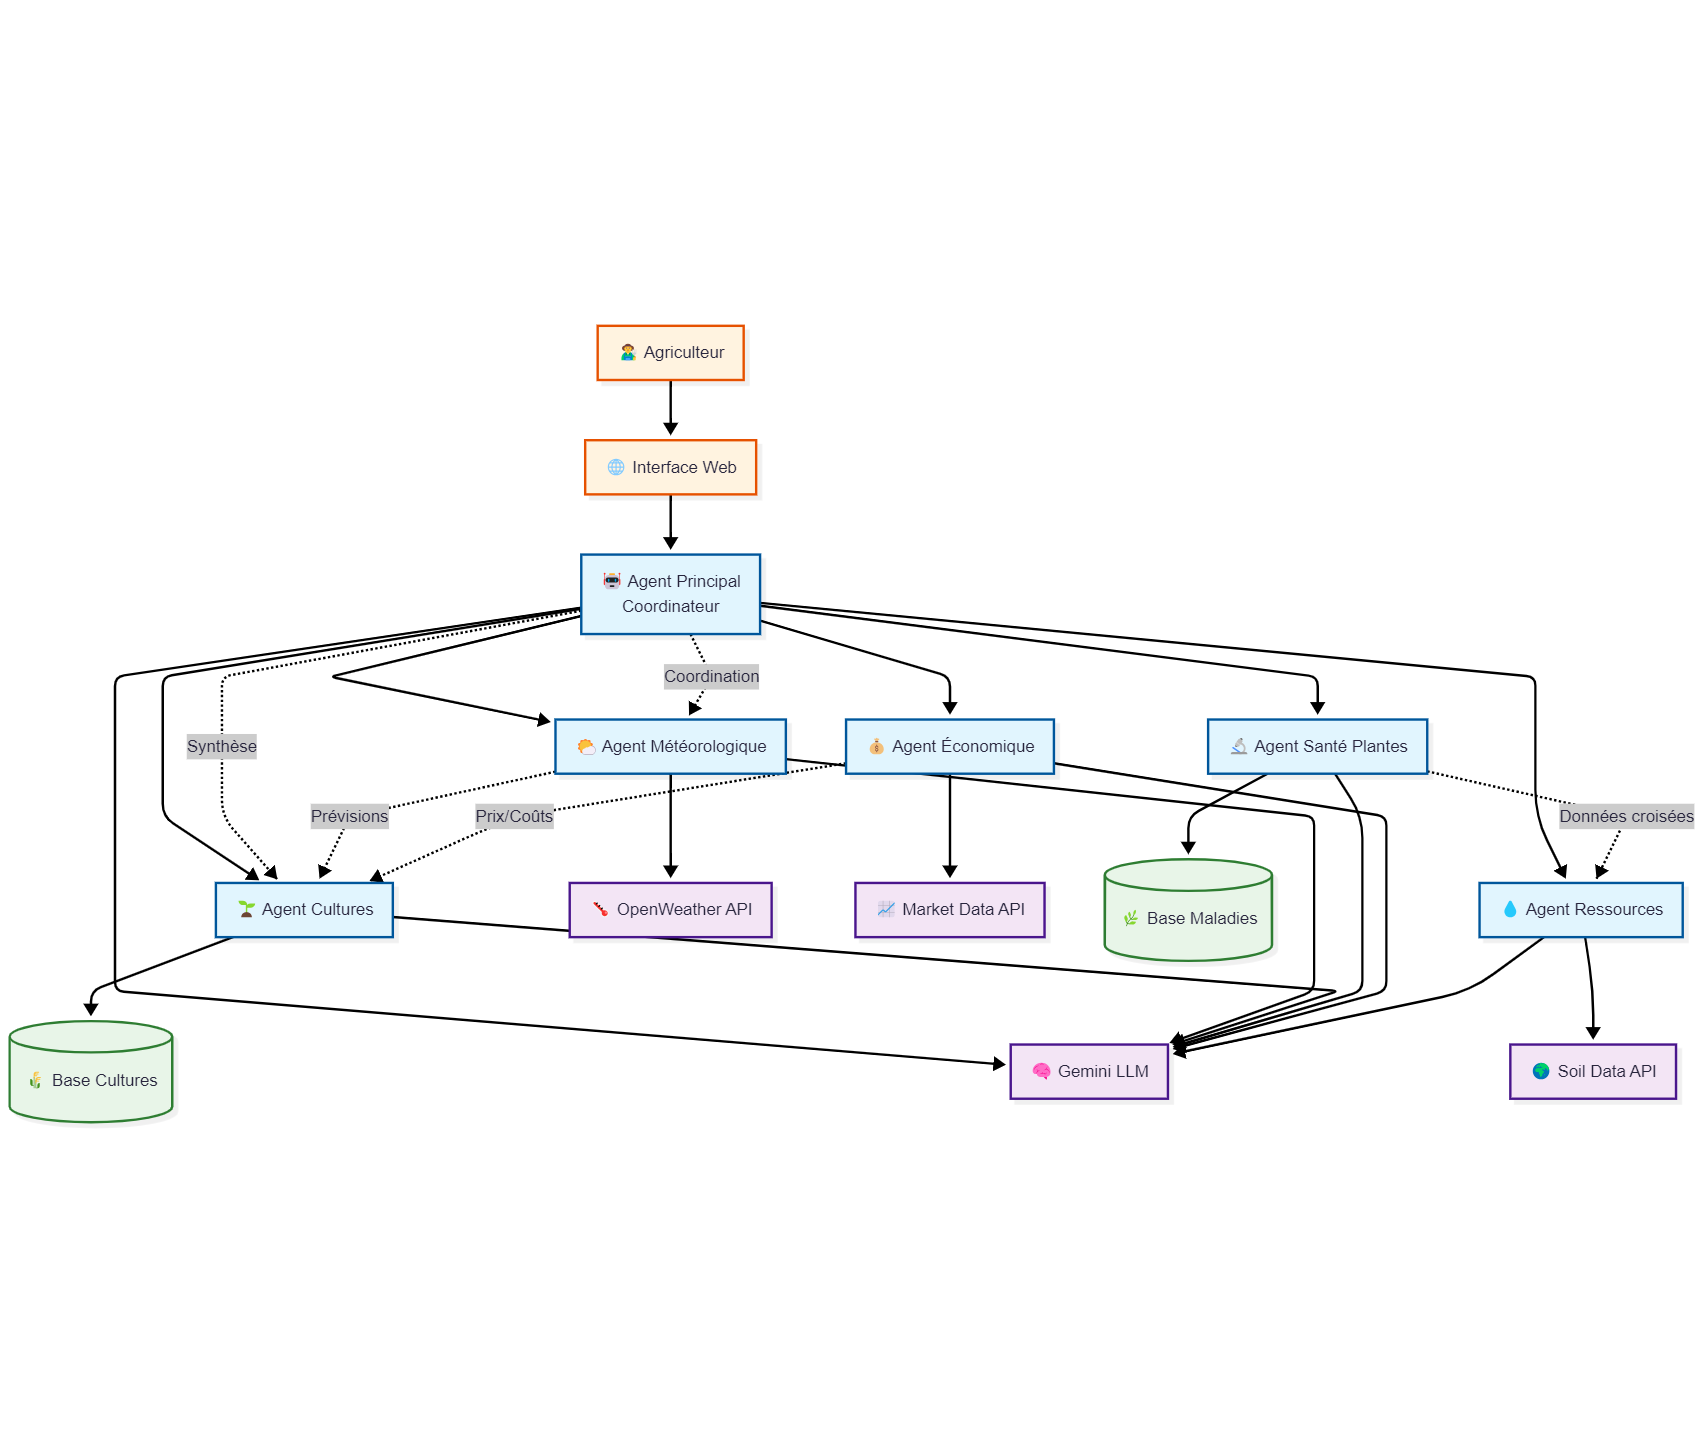
\includegraphics[width=0.9\textwidth]{images/architectures.png}
\caption{Architecture multi-agents du système Agriculture Cameroun avec flux de communication}
\label{fig:architecture}
\end{figure}

Le diagramme d'architecture présenté dans la Figure \ref{fig:architecture} illustre l'organisation hiérarchique du système Agriculture Cameroun selon une structure en arbre descendant. Au sommet, l'Agriculteur (👨‍🌾) représente l'utilisateur final du système, point d'entrée unique pour toutes les interactions. Cette représentation souligne l'approche centrée utilisateur du système, conçu spécifiquement pour les producteurs agricoles camerounais.

L'Interface Web (🌐) constitue la couche de présentation, offrant une interface intuitive et accessible via navigateur web. Cette interface traduit les requêtes utilisateur en formats structurés et présente les réponses des agents de manière claire et actionnable. Son positionnement direct sous l'utilisateur illustre son rôle de pont entre l'humain et le système multi-agents.

L'Agent Principal Coordinateur (🤖) occupe une position centrale stratégique dans l'architecture. Représenté par l'icône robot avec le sous-titre "Coordinateur", il incarne le cerveau du système, responsable de l'orchestration de tous les agents spécialisés. Les connexions directes descendantes vers les cinq agents spécialisés illustrent sa capacité de routage intelligent et de coordination des requêtes complexes.

Les cinq agents spécialisés sont organisés horizontalement sous l'Agent Principal, chacun identifié par une icône métier distinctive. L'Agent Météorologique (🌤️) gère les prévisions et analyses climatiques. L'Agent Cultures (🌱) traite les questions liées aux variétés, plantations et cycles agricoles. L'Agent Santé des Plantes (🔬) se spécialise dans le diagnostic et le traitement des maladies. L'Agent Économique (💰) analyse la rentabilité et les tendances de marché. L'Agent Ressources (💧) optimise la gestion de l'eau, du sol et des intrants.

La couche externe du diagramme présente l'écosystème de données et services. Chaque agent spécialisé maintient des connexions dédiées vers ses sources d'information : l'Agent Météorologique se connecte à l'OpenWeather API (🌡️), l'Agent Économique aux Market Data API (📈), tandis que les autres agents accèdent à des bases de données spécialisées représentées par des cylindres : Base Maladies (🌿), Base Cultures (🌾), et Soil Data API (🌍).

L'intégration du LLM Gemini (🧠) constitue un élément architectural innovant. Connecté à l'Agent Principal et aux cinq agents spécialisés, Gemini enrichit le système de capacités de traitement du langage naturel et de raisonnement avancé, permettant des analyses contextuelles sophistiquées et des réponses en langage naturel.

Les flux de communication inter-agents, représentés par des lignes pointillées annotées, illustrent la capacité de collaboration directe entre agents. Les connexions "Coordination" et "Synthèse" depuis l'Agent Principal, ainsi que les échanges "Données croisées", "Prévisions" et "Prix/Coûts" entre agents spécialisés, démontrent l'intelligence distribuée du système et sa capacité d'optimisation collaborative.


\section{Scénarios d'Interaction}

\subsection{Cas d'usage : Consultation météorologique}

Le scénario de consultation météorologique illustre parfaitement la valeur ajoutée du système multi-agents dans la transformation d'une simple requête d'information en conseil agricole actionnable. Considérons le cas de Mama Félicité, une productrice de tomates de la région du Centre, qui s'inquiète des pluies annoncées pour la semaine alors que ses tomates approchent de la maturité.

Mama Félicité formule sa requête en langage naturel, mélangeant français et expressions locales comme c'est courant : "Mes tomates go bientôt mûrir, est-ce que les pluies de cette semaine vont gâter ma récolte ?". L'interface utilisateur capture cette requête et la transmet à l'Agent Coordinateur Principal qui immédiatement identifie la nature composite de la question, impliquant des aspects météorologiques, culturaux et potentiellement économiques.

L'Agent Coordinateur décompose intelligemment la requête en plusieurs sous-questions. Il sollicite d'abord l'Agent Météorologique pour obtenir les prévisions détaillées de la semaine, avec une attention particulière sur l'intensité et la durée des précipitations prévues. Simultanément, il interroge l'Agent Cultures sur le stade de maturité des tomates et leur vulnérabilité aux pluies à ce stade. Anticipant les besoins de Mama Félicité, il consulte également l'Agent Économique sur l'évolution probable des prix des tomates dans les jours à venir.

L'Agent Météorologique analyse les données disponibles et fournit une réponse nuancée. Les prévisions indiquent des pluies modérées à fortes pendant trois jours à partir de jeudi, avec des accalmies en matinée. L'agent ne se contente pas de fournir ces données brutes mais les contextualise pour l'agriculture, notant que l'intensité prévue présente un risque significatif pour les tomates mûres exposées.

L'Agent Cultures, informé du stade de maturité des tomates, évalue les risques spécifiques. Les tomates proches de la maturité sont particulièrement vulnérables à l'éclatement et aux maladies fongiques en cas de pluies intenses. L'agent calcule qu'environ 40\% de la récolte pourrait être affectée si aucune mesure n'est prise, mais propose plusieurs stratégies d'atténuation incluant la récolte anticipée des fruits les plus mûrs, l'installation de bâches protectrices sur les plants les plus exposés, et l'application préventive de fongicides biologiques.

L'Agent Économique apporte une dimension stratégique cruciale en analysant les tendances du marché. Les prix actuels sont stables mais pourraient augmenter de 15-20\ après les pluies en raison des pertes anticipées chez d'autres producteurs. Cependant, les tomates récoltées légèrement avant maturité complète se vendront 10\% moins cher. L'agent fournit une analyse coût-bénéfice détaillée des différentes options.

L'Agent Coordinateur Principal synthétise ces informations en une réponse cohérente et actionnnable pour Mama Félicité. La recommandation finale suggère une stratégie mixte : récolter immédiatement 60\% des tomates les plus mûres pour les vendre au prix actuel, protéger 30\% des plants avec des bâches pour une récolte post-pluie à prix premium, et accepter un risque calculé sur les 10\% restants. Cette stratégie optimise le revenu total tout en minimisant les pertes potentielles.

La réponse inclut également un calendrier d'action détaillé : mardi et mercredi pour la récolte sélective et la vente, mercredi soir pour l'installation des protections, et jeudi matin pour l'application de traitements préventifs. Le système programme même des rappels pour chaque action et propose un suivi post-pluie pour évaluer l'état des plants protégés.

\subsection{Cas d'usage : Diagnostic de maladie}

Le diagnostic de maladie représente l'un des scénarios les plus critiques où le système démontre sa capacité à potentiellement sauver des récoltes entières. Prenons l'exemple de Papa Jean, un producteur de cacao de la région du Sud, qui observe avec inquiétude des taches brunes suspectes sur ses cabosses accompagnées d'un flétrissement inhabituel de certaines branches.

Papa Jean décrit ses observations au système : "J'ai des taches marron sur mes cabosses de cacao et certaines branches commencent à sécher. Ça a commencé il y a une semaine après les fortes pluies". Cette description, bien que simple, contient plusieurs indices diagnostiques que l'Agent Coordinateur Principal identifie immédiatement comme nécessitant une investigation approfondie.

L'Agent Santé des Plantes prend immédiatement le lead sur cette requête, initiant un processus de diagnostic différentiel sophistiqué. L'agent commence par analyser les symptômes décrits en les comparant à sa base de données extensive de maladies du cacao. La combinaison de taches brunes sur cabosses et de dessèchement de branches, particulièrement après des pluies intenses, évoque plusieurs possibilités incluant la pourriture brune (Phytophthora), les attaques de mirides, ou potentiellement une combinaison de problèmes.

Pour affiner le diagnostic, l'Agent Santé des Plantes engage un dialogue interactif avec Papa Jean, posant des questions ciblées sur la localisation des taches (base, milieu ou sommet des cabosses), leur évolution (croissance rapide ou lente), la présence d'exsudats ou de sporulation, et l'étendue du problème dans la plantation. Chaque réponse permet à l'agent d'ajuster ses hypothèses diagnostiques en temps réel.

Parallèlement, l'Agent Météorologique est consulté pour analyser les conditions climatiques récentes. L'agent confirme que les conditions d'humidité élevée et de température modérée des deux dernières semaines ont créé un environnement optimal pour le développement de maladies fongiques, renforçant l'hypothèse de la pourriture brune.

L'Agent Cultures apporte des informations contextuelles cruciales en notant que la variété de cacao cultivée par Papa Jean est modérément sensible à la pourriture brune et que la densité de plantation relativement élevée dans sa parcelle peut avoir favorisé la propagation de la maladie en limitant la circulation d'air.

Après cette analyse multi-dimensionnelle, l'Agent Santé des Plantes établit un diagnostic de pourriture brune avec un niveau de confiance de 85\%, tout en maintenant une vigilance sur la possibilité d'une infection secondaire par des mirides profitant de l'affaiblissement des plants. L'agent propose immédiatement un plan de traitement intégré comprenant des mesures curatives d'urgence et des stratégies préventives à long terme.

Le plan de traitement immédiat inclut l'élimination et la destruction de toutes les cabosses infectées pour réduire l'inoculum, l'application d'un fongicide à base de cuivre avec des instructions précises sur le dosage et la technique d'application, et l'amélioration urgente du drainage dans les zones les plus affectées. L'Agent Économique est sollicité pour calculer le coût de ces interventions et confirmer leur viabilité économique compte tenu de la valeur de la récolte à sauver.

Pour le long terme, le système recommande un programme de gestion intégrée incluant la taille sanitaire pour améliorer l'aération, l'introduction progressive de variétés plus résistantes, et un calendrier de traitements préventifs aligné sur les périodes à risque identifiées par l'Agent Météorologique. L'Agent Ressources contribue en suggérant des amendements du sol pour renforcer la résistance naturelle des plants.

Le système ne s'arrête pas à la fourniture de recommandations mais établit un protocole de suivi. Des rappels sont programmés pour vérifier l'évolution de la situation, et Papa Jean est invité à fournir des mises à jour régulières permettant d'ajuster le traitement si nécessaire. Cette approche itérative assure une gestion optimale de la crise phytosanitaire.

\subsection{Cas d'usage : Analyse économique}

L'analyse économique représente un domaine où le système multi-agents transforme des données complexes en insights stratégiques accessibles. Illustrons cela avec le cas de la Coopérative des Planteurs Unis de Bafoussam, qui envisage de diversifier sa production actuellement centrée sur le café arabica vers l'inclusion de cultures maraîchères pour optimiser ses revenus.

Le président de la coopérative, M. Kamga, soumet une requête complexe au système : "Notre coopérative cultive 50 hectares de café arabica mais les prix fluctuent beaucoup. Nous pensons à utiliser 10 hectares pour des légumes. Qu'est-ce qui serait le plus rentable ?". Cette question apparemment simple cache une complexité considérable nécessitant l'expertise coordonnée de plusieurs agents.

L'Agent Coordinateur Principal reconnaît immédiatement la nature stratégique de cette requête et mobilise une équipe d'agents pour conduire une analyse complète. L'Agent Économique prend naturellement le lead mais travaille en étroite collaboration avec les Agents Cultures, Météorologique et Ressources pour fournir une analyse holistique.

L'Agent Économique commence par analyser la situation actuelle de la coopérative. Les données historiques montrent que le café arabica a généré des revenus moyens de 2,5 millions FCFA par hectare sur les trois dernières années, avec une volatilité importante (écart-type de 600,000 FCFA). L'agent identifie que cette volatilité est principalement due aux fluctuations des prix internationaux sur lesquels la coopérative n'a aucun contrôle.

Pour l'analyse de diversification, l'Agent Économique collabore étroitement avec l'Agent Cultures pour identifier les options maraîchères les plus prometteuses. L'Agent Cultures, considérant les conditions agro-climatiques de Bafoussam, la disponibilité de main-d'œuvre et l'accès aux marchés, recommande trois scénarios de diversification : tomates et poivrons en rotation, pommes de terre suivies de choux, ou un mix de légumes-feuilles à cycle court.

L'Agent Météorologique apporte des insights critiques en analysant les patterns climatiques de Bafoussam et leur évolution probable. Les données montrent que la région bénéficie de conditions favorables pour le maraîchage avec deux saisons de production possibles, mais avec des risques de grêle croissants en altitude qui pourraient affecter certaines cultures.

L'Agent Ressources évalue les implications en termes de besoins en eau, en main-d'œuvre et en intrants pour chaque scénario. Le maraîchage nécessite une irrigation plus intensive que le café, mais les infrastructures existantes de la coopérative peuvent être adaptées. La main-d'œuvre additionnelle nécessaire est estimée et chiffrée.

L'Agent Économique synthétise toutes ces informations dans une analyse financière détaillée. Pour le scénario tomates-poivrons, les projections montrent un revenu potentiel de 4,2 millions FCFA par hectare avec une volatilité réduite car basée sur les marchés locaux. Le scénario pommes de terre-choux offre 3,8 millions FCFA par hectare mais avec une meilleure résilience aux aléas climatiques. Le mix de légumes-feuilles génère 3,5 millions FCFA mais avec l'avantage de revenus réguliers tout au long de l'année.

L'analyse ne s'arrête pas aux chiffres bruts. L'Agent Économique modélise différents scénarios de transition, montrant l'impact de convertir 5, 10 ou 15 hectares sur les revenus totaux et la stabilité financière de la coopérative. L'analyse de risque montre que la diversification avec 10 hectares de tomates-poivrons réduirait la volatilité globale des revenus de 40\% tout en augmentant le revenu moyen de 15\%.

Le système produit également une feuille de route détaillée pour la mise en œuvre, incluant le calendrier optimal de transition pour minimiser les perturbations, les investissements nécessaires en infrastructure et leur période de retour sur investissement, les besoins en formation pour les membres de la coopérative, et les stratégies de commercialisation pour les nouveaux produits.

L'Agent Coordinateur Principal présente ces résultats sous forme de tableaux comparatifs clairs, de graphiques de projection et de recommandations priorisées. La recommandation finale suggère une approche progressive : commencer avec 5 hectares de tomates-poivrons la première année pour tester et affiner le modèle, puis étendre à 10 hectares si les résultats sont conformes aux projections.

\subsection{Diagrammes de séquence annotés}

\begin{figure}[H]
\centering
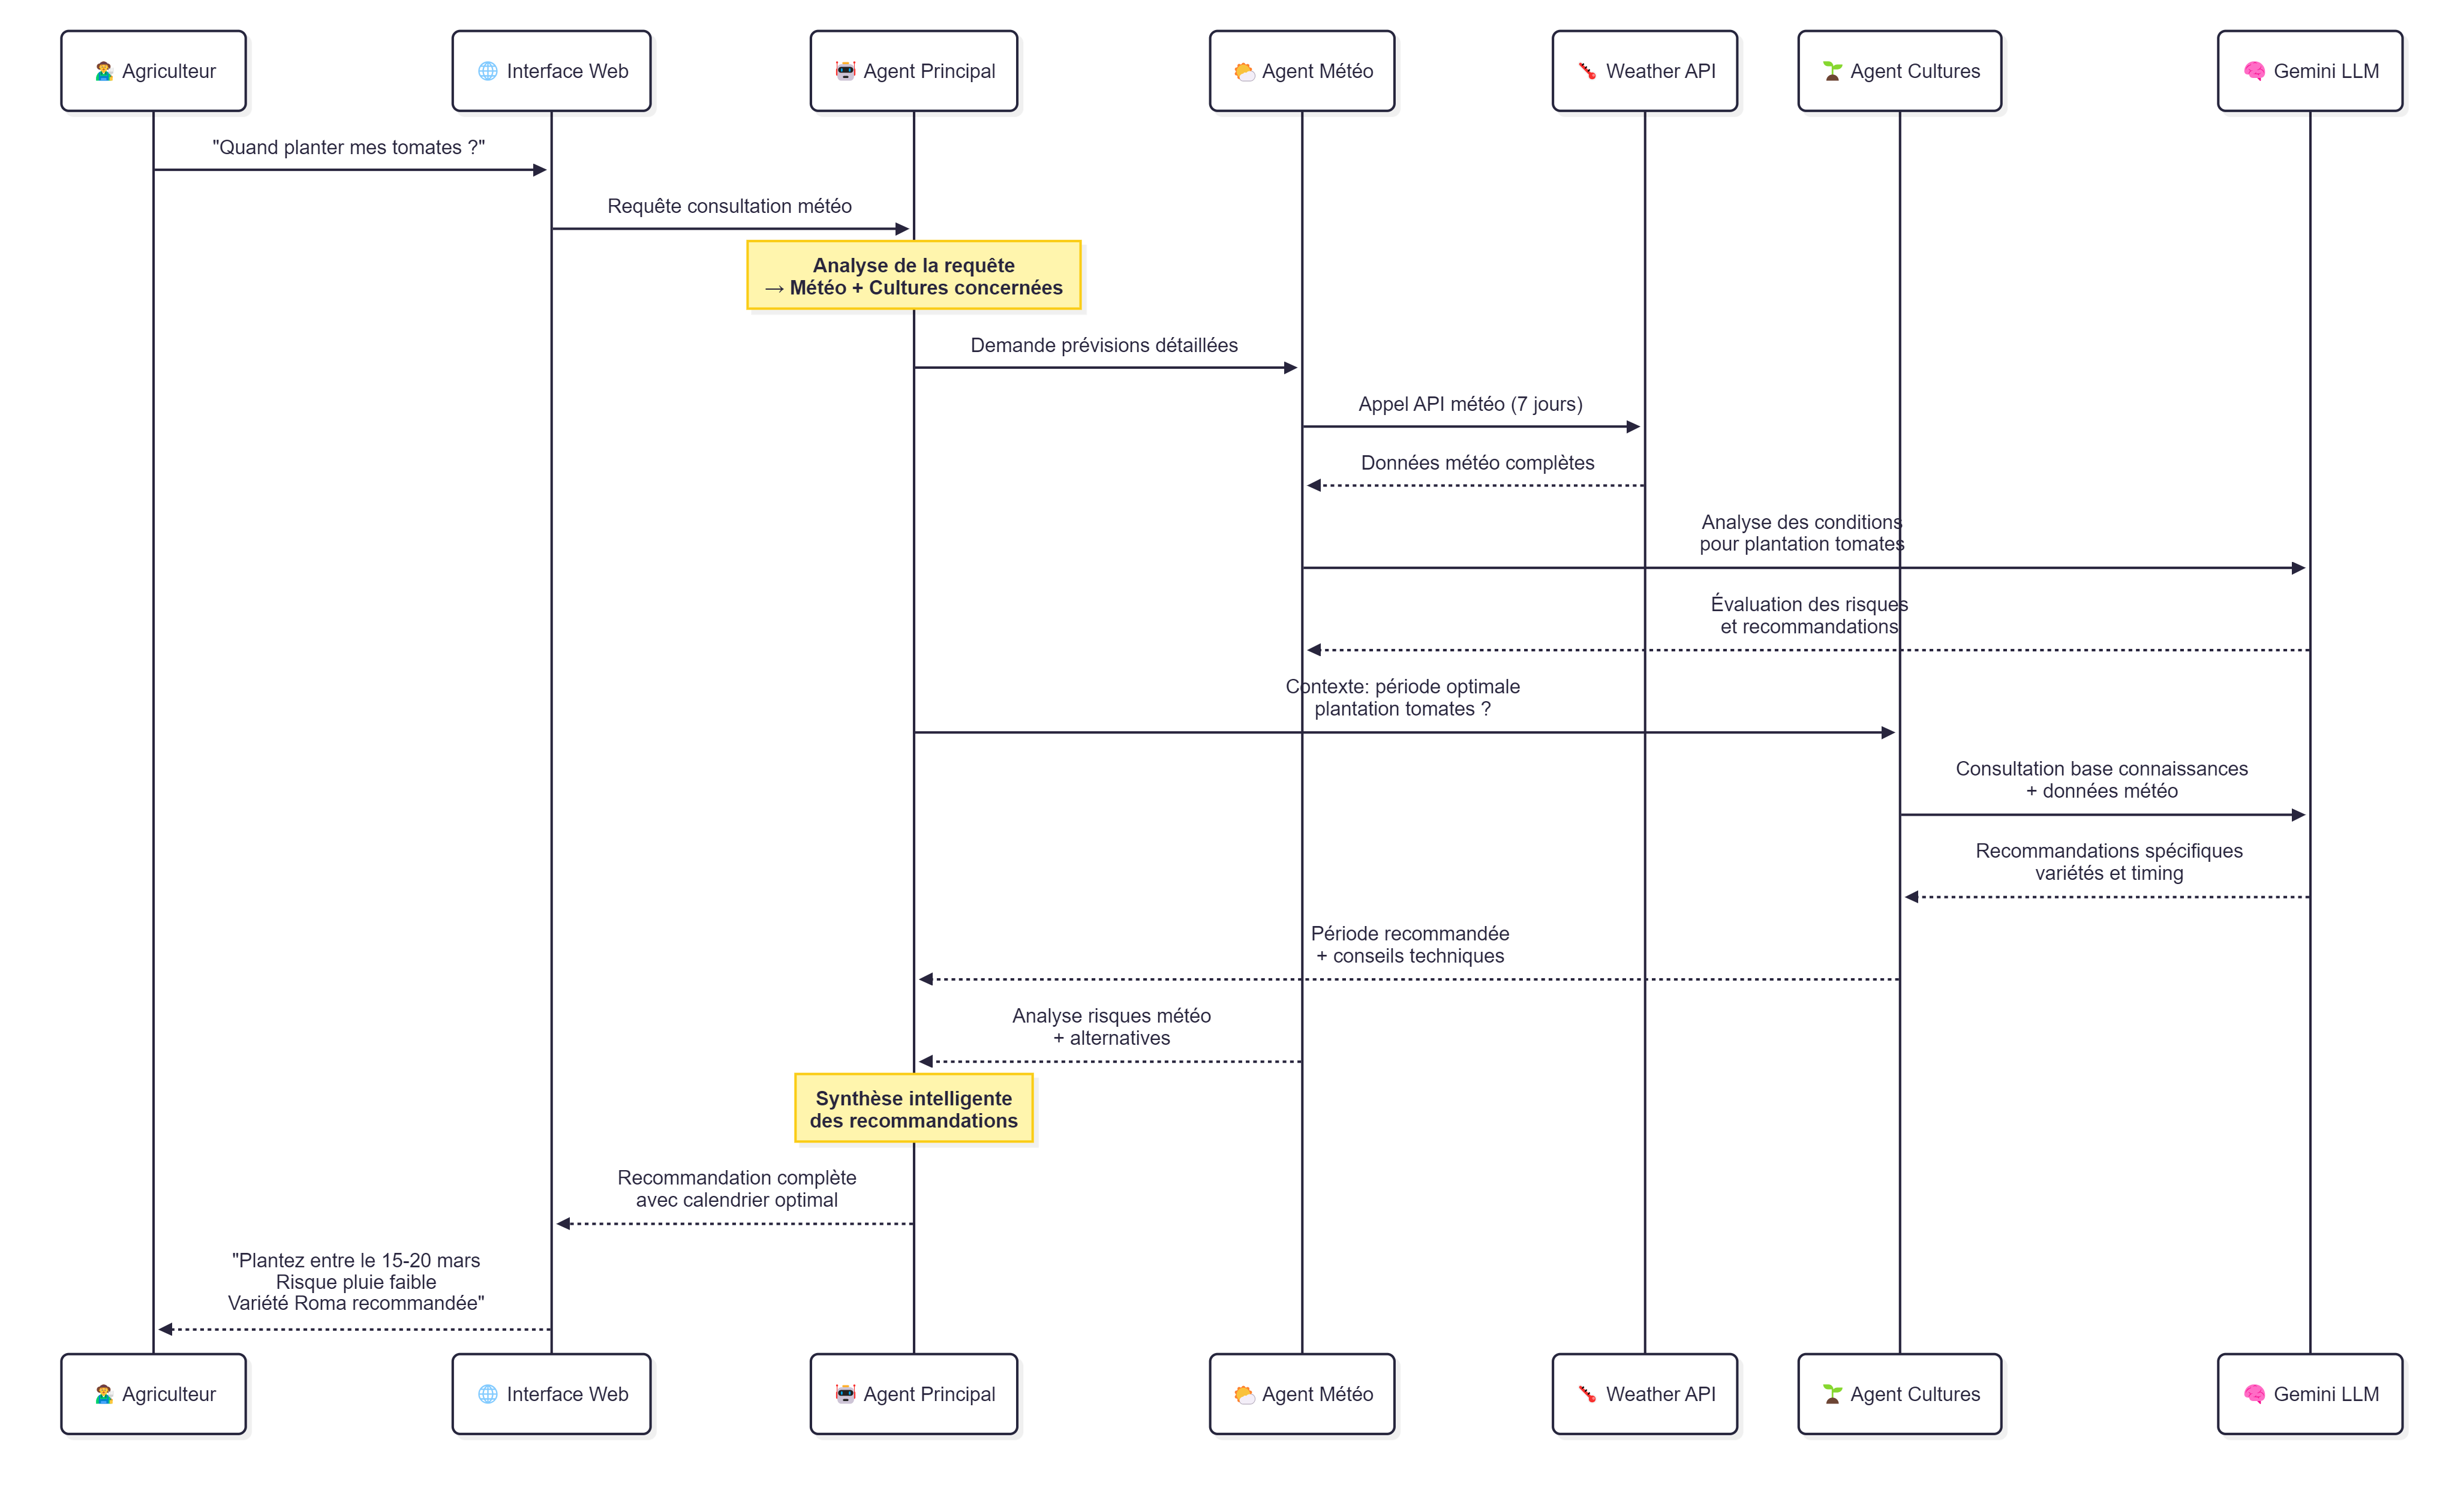
\includegraphics[width=0.95\textwidth]{images/sequence_diagram_weather.png}
\caption{Diagramme de séquence pour une consultation météorologique complexe}
\label{fig:sequence_weather}
\end{figure}

Le diagramme de séquence présenté dans la Figure \ref{fig:sequence_weather} illustre le flux d'interactions pour une consultation météorologique complexe. La séquence commence par l'utilisateur (représenté par l'icône d'agriculteur) qui formule sa requête en langage naturel vers l'interface utilisateur. Cette interface, symbolisée par un écran de dialogue, effectue une première analyse syntaxique et transmet la requête structurée à l'Agent Coordinateur Principal.

L'Agent Coordinateur, représenté au centre du diagramme, décompose la requête en identifiant les différentes dimensions du besoin. Les flèches annotées montrent comment il génère des sous-requêtes spécifiques : une demande de prévisions détaillées vers l'Agent Météorologique, une requête sur la sensibilité des cultures vers l'Agent Cultures, et une analyse d'impact économique vers l'Agent Économique.

Les interactions parallèles sont représentées par des barres d'activation simultanées, montrant comment les agents spécialisés travaillent en parallèle pour optimiser le temps de réponse. L'Agent Météorologique consulte ses sources de données externes (représentées par des appels asynchrones en pointillés) avant de retourner ses prévisions enrichies.

Les annotations sur les flèches de retour indiquent le type et le contenu des réponses. L'Agent Météorologique retourne non seulement les données brutes mais aussi une évaluation des risques. L'Agent Cultures fournit des seuils critiques et des recommandations préventives. L'Agent Économique apporte une analyse coût-bénéfice des différentes options.

La phase de synthèse est représentée par une boîte d'activation étendue sur l'Agent Coordinateur, illustrant le processus complexe d'intégration et d'harmonisation des différentes réponses. Les conflits potentiels et leur résolution sont annotés, montrant par exemple comment une recommandation de récolte précoce de l'Agent Cultures est pondérée par l'analyse de prix de l'Agent Économique.

\begin{figure}[H]
\centering
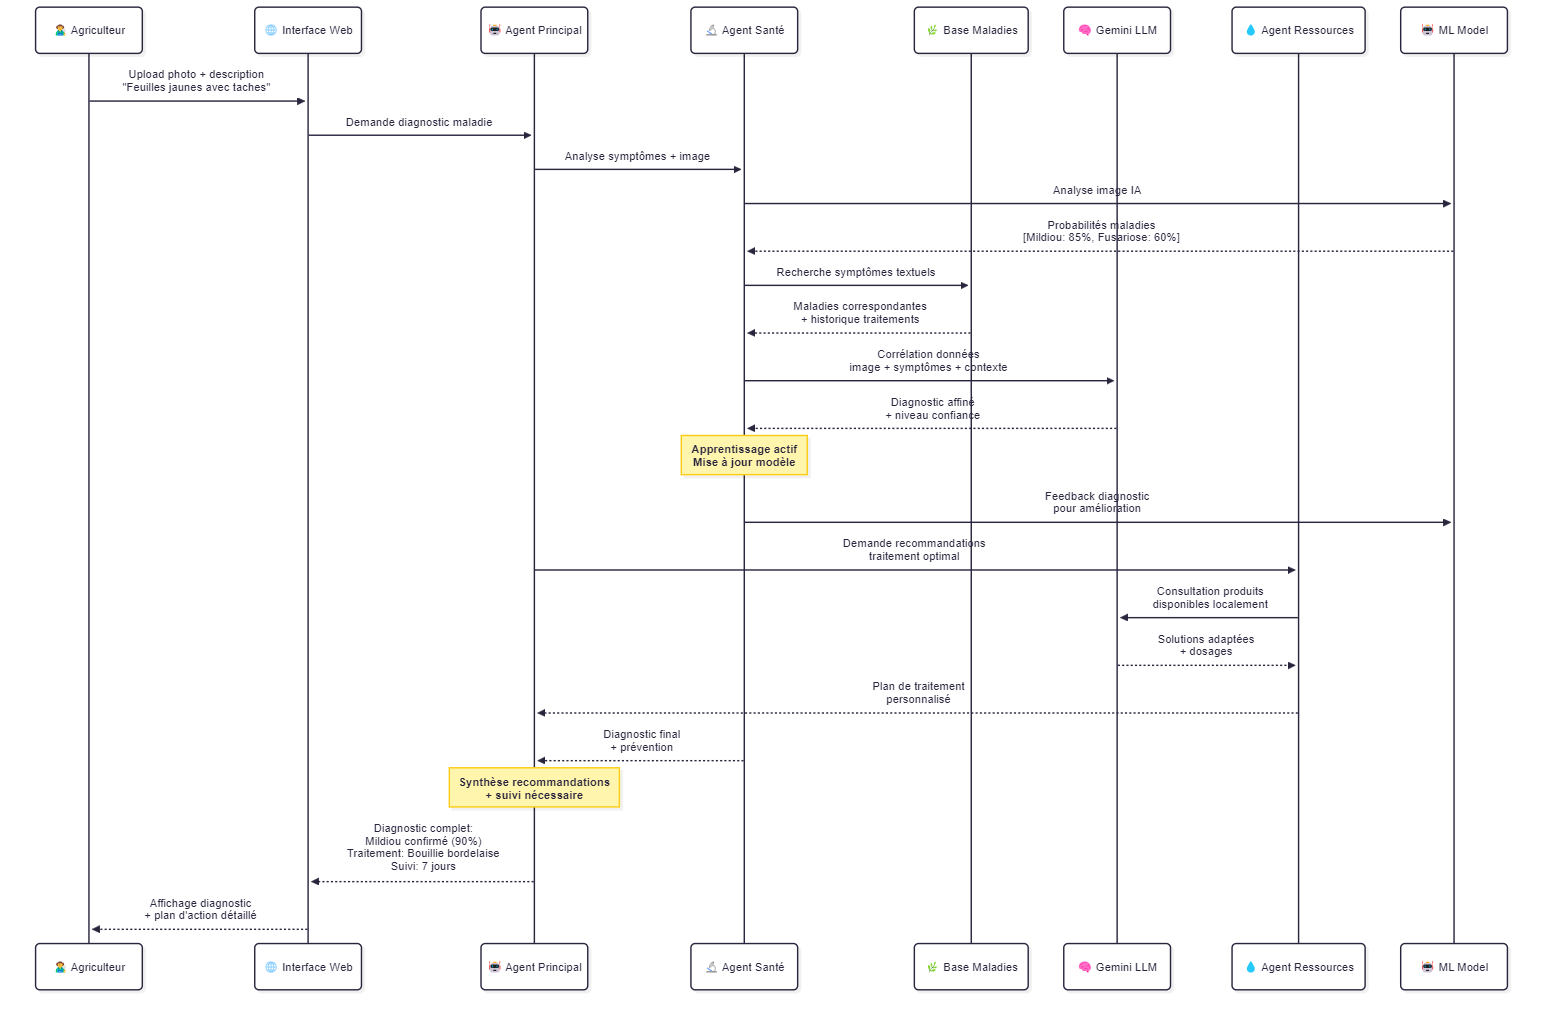
\includegraphics[width=0.95\textwidth]{images/sequence_diagram_disease.png}
\caption{Diagramme de séquence pour un diagnostic de maladie avec apprentissage}
\label{fig:sequence_disease}
\end{figure}

La Figure \ref{fig:sequence_disease} présente un scénario plus complexe de diagnostic de maladie impliquant des interactions itératives et des mécanismes d'apprentissage. Le diagramme montre comment l'Agent Santé des Plantes mène l'investigation en sollicitant activement des informations complémentaires.

Les boucles de dialogue sont représentées par des rectangles annotés "Loop" avec leurs conditions de sortie. L'Agent Santé des Plantes pose des questions diagnostiques successives jusqu'à atteindre un niveau de confiance suffisant (>80\%) ou épuiser les questions pertinentes. Chaque itération enrichit le contexte et affine le diagnostic.

Les consultations croisées entre agents sont mises en évidence par des flèches horizontales entre les lignes de vie des agents. L'Agent Santé consulte l'Agent Météorologique pour comprendre les conditions favorisant la maladie, et l'Agent Cultures pour obtenir l'historique cultural et la sensibilité variétale.

Le mécanisme d'apprentissage est représenté par des flèches en retour vers une base de connaissances (cylindre de données). Après confirmation du diagnostic par l'utilisateur, le système met à jour ses modèles pour améliorer les futures diagnostics similaires. Cette rétroaction est annotée comme "Apprentissage confirmé" avec les paramètres mis à jour.

\begin{figure}[H]
\centering
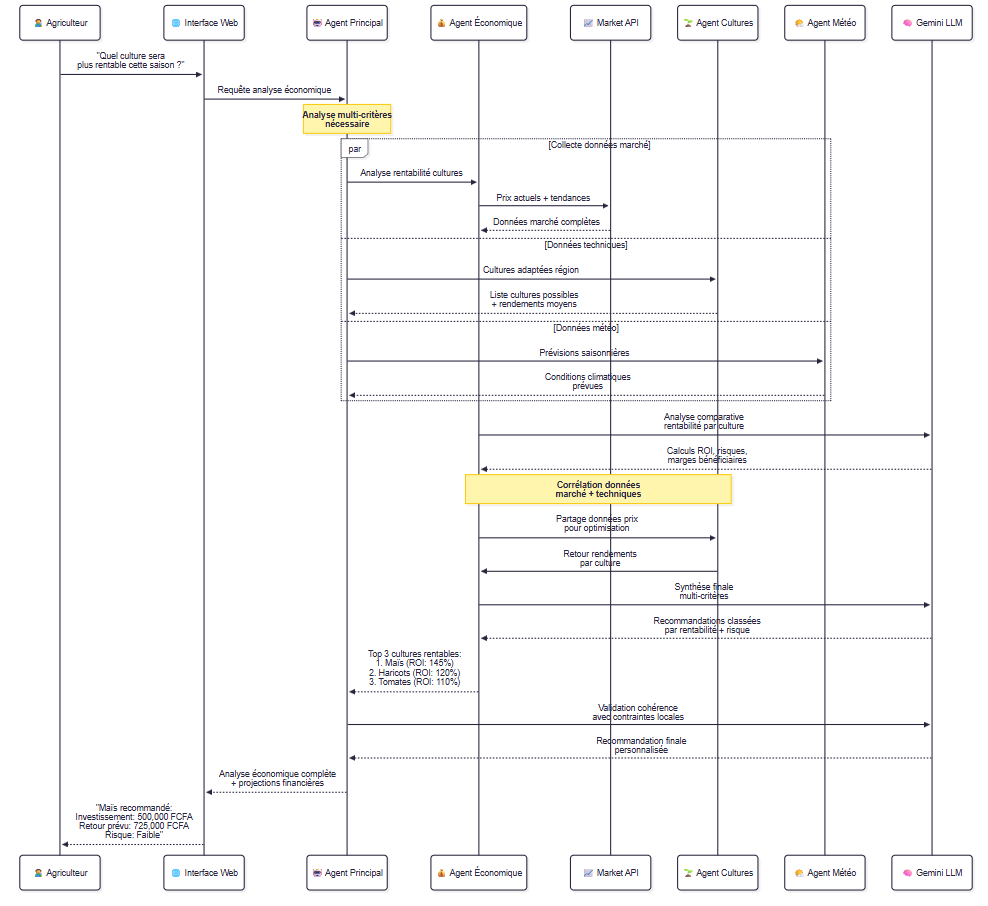
\includegraphics[width=1\textwidth]{images/sequence_diagram_economic.png}
\caption{Diagramme de séquence pour une analyse économique multi-critères}
\label{fig:sequence_economic}
\end{figure}

La Figure \ref{fig:sequence_economic} illustre la complexité d'une analyse économique impliquant tous les agents du système. Le diagramme met en évidence la nature hautement collaborative de ce type de requête, avec de multiples allers-retours entre agents pour affiner l'analyse.

La phase d'initialisation montre l'Agent Économique établissant le contexte d'analyse en sollicitant des informations de base de tous les autres agents. Cette phase est représentée par un éventail de flèches partant de l'Agent Économique, chacune annotée avec le type d'information demandée.

Les calculs parallèles sont représentés par des boîtes d'activation simultanées sur plusieurs agents. Pendant que l'Agent Économique modélise les scénarios financiers, l'Agent Cultures évalue les implications techniques de chaque option, l'Agent Météorologique analyse les risques climatiques, et l'Agent Ressources calcule les besoins en intrants.

Les points de synchronisation sont clairement marqués par des lignes horizontales annotées "Sync", montrant où les différents flux d'analyse doivent converger avant de progresser. Ces points correspondent aux moments où l'Agent Coordinateur consolide les résultats intermédiaires pour vérifier la cohérence et identifier les éventuels besoins d'analyse supplémentaire.

La présentation finale des résultats est détaillée dans une note attachée au message de retour vers l'utilisateur, spécifiant le format multi-modal de la réponse incluant tableaux comparatifs, graphiques de projection et recommandations textuelles structurées.
